\section{Concrete approaches}\label{approaches}
\subsection{Narratology excursion}
The following two subsections (\ref{fabula} and \ref{discourse}) will showcase two concrete cases of story telling by application of AI planning. Because they approach the subject matter on different levels a distiction is required. It will be necessary to distinguish between \emph{fabula} (or \emph{story}) on the one hand, and \emph{discourse} (or \emph{plot}) on the other hand.\\
Chatman writes in \cite{Chatman1980} (furthermore cited in \cite{Herman10}):
\begin{quote}
''In simple terms, the story is the \emph{what} in a narrative that is depicted, discourse is the \emph{how}.''

(Note: Since \emph{story} and \emph{plot} are more commonly used in everyday language and might lead to confusion or wrong assumptions the remainder of this document will refer to the two concepts as \emph{fabula} and \emph{discourse}.)
\end{quote}
To illustrate the difference with an example: viewers of a movie might be presented with a character A, talking about what a character B has done (assume A's report to be truthful and B's action to be relevant for the movie). On the level of the fabula (the narrative structure), we have B doing something. On the level of the discourse (how this is conveyed to the recipient) we have A talking about it. When watching a movie or reading a book one is presented with a discourse and automatically constructs a fabula in their head.
% - 2 approaches address story/narrative at different levels
% - fabula vs discourse
\subsection{Planning a fabula}\label{fabula}
In \cite{Haslum14} Haslum shows how a specific model of story generation proposed for the IPOCL planner\cite{Riedl10} can be compiled into a classic planning problem. The model in question is designed to create fabulae and incorporates the notion of character intetions. The following subsection will describe the story world modeling in general. After that aforementioned compilation will be adressed.

\subsubsection{Story world modeling}
The central building blocks in this apporach are story characters for which certain abilities are defined. For illustration purposes a story world which is loosely based on the tale of Aladdin is used. Characters are humans (Aladdin, Jasmine, king Jafar) and monsters (a genie, a dragon). The characters' abilities are actions which can be divided into intentional actions and happenings. The former are deliberate interactions with the story world or other characters (such as traveling between locations or slaying a monster) while the latter are unintentional effects (e.g. a monster scaring a human because of its appearance or a human falling in love with another).

In order to create coherent, believable fabulae the modeling lays its focus on intentionality. Apart from the desired story outcome (the goal of the overall planning problem) characters can have their own goals which can arise and change through influence by the story world. Intentionality can also be caused by delegation --- i.e. a character $A$ evokes a character goal in another character $B$ (for example through a command or persuasion). Most importantly character goals allow for \emph{intentional plans} which characters can pursue. When a character has a goal and carries out an action in order to reach it, the action is said to be performed in a \emph{frame of commitment}. Formally these terms are defined as follows:
\begin{quote}
''\textbf{Definition 1} An intentional plan is one in which every occurrence of an intentional action is part of some frame of commitment. A frame of commitment is a subset $S'$ of steps (i.e., action occurrences) in the plan, associated with a modal literal $(intends\ A\ g)$, satisfying four requirements: (1) Character $A$ is an actor of every step in $S'$. (2) There is a final step $s_{fin}\in S'$ that makes $g$ true. (3) There is a motivating step $s_m$ in the plan, which adds $(intends\ A\ g)$ and which precedes all steps in $S'$. We’ll say there is a motivational link from $s_m$ to every step in the frame of commitment, $S'$. Note that $s_m$ is not part of $S'$. (4) From each step in $S'$ other than $s_{fin}$ there is a path of causal or motivational links to $s_{fin}$. A complete (fabula) plan is one that is both intentional and valid in the classical sense.'' \cite{Haslum14}
\end{quote}
To visually aid the formal definition consider figure \ref{fig:intplan} on page \pageref{fig:intplan}. Arrows are to represent actions and dashed lines an arbitrary sequence of actions not shown. If all blue arrows are actions carried out by character $A$ then the frame of commitment is $S'=\{s_i,s_{i+1},s_{i+x},s_{fin}\}$. Note that $s_m$ does not necessarily have to be an action of $A$ since intention can be delegated and that the intentional plan which includes $S'$ may contain an arbitrary number of happenings unrelated to $S'$ or $g$.
\begin{figure}[htbp]
 \centering
 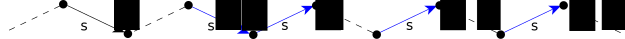
\includegraphics[scale=0.8]{intentional_plan}
 \caption{Visual example of a frame of commitment.}
 \label{fig:intplan}
\end{figure}

Ensuring that character goals are pursued by means of intentional plans is referred to as \emph{explicit justification tracking}. In \cite{Riedl10} this is performed by the IPOCL planner but in \cite{Haslum14} it is incorporated into the planning problem. This is accomplished by the main compilation described in \cite{Haslum14} and will be briefly discussed in the following subsection.

% - (desired) story outcome
% - character goals (can change, are influenced by other characters / events)
% - intentional agents (actions percievable as contributing to goals)
% - characters (humans, monsters (genie, dragon))
%     - have given abilities (travel betw. locations, slay monsters, take things from dead, gain control over (genie), fall in love, marry)
%     -> move in world, interact w/ other chars + world/objects
% - intentional actions vs. happenings (e.g. monster frightens human, human falls in love)
% - delegating actions (command, persuade, bribe, ... other char to so sth.)
% - intentional plan
%     -> frame of commitment
% - 
% - 
\subsubsection{Compilation}
The original story generation model includes modal literals in the form of $(intends\ A\ g)$ in order to handle intentionality. For the compilation into a classic planning problem predicates are introduced for intention, delegation and justification. Intention literals are used as preconditions for intentional actions, which allows the modeling of frames of commitment --- e.g. $(intends\h dead\ Aladdin\ Dragon)$ as a precondition for every action in Aladdins frame of commitment to slay the dragon including the $s_{fin}$ of him achieving his goal. Delegation and justification literals, on the other hand, are used for justification tracking. They are true in the initial state, required to be true at the goal, made false by certain intentional actions and then set up in a way such that only if motivational link as described in Definition 1 are adhered to will they become true again.

Description and discussion of this compilation's precise nature take up most of \cite{Haslum14} and can therefore not be covered here. To get an intuition of a possible output consider below example of a monster slaying action in PPDL-like syntax.
\begin{lstlisting}[frame=single,basicstyle=\scriptsize,numbers=left,numberstyle=\tiny]
(:action slay-1-because-intends-dead
    :parameters (?knight - knight ?monster - monster ?where - place)
    :precondition (and (alive ?knight) (at ?knight ?where)
                       (alive ?monster) (at ?monster ?where)
                       (intends ?knight (dead ?monster))
                  (not (exists (?c) (and (not (= ?c ?knight))
                                         (delegated ?c (dead ?monster))))))
    :effect (and (not (alive ?monster)) (dead ?monster)
        (justified (at ?knight ?where) (intends ?knight (dead ?monster)))
        (justified (at ?monster ?where) (intends ?knight (dead ?monster)))
        (not (delegated ?knight (dead ?monster)))))
\end{lstlisting}
A notable restriction of the compilation is that a delegated goal can only be achieved by the character it has been delegated to. In case of above monster slaying example this can be seen in lines 6 and 7. The monster may only be slain if there exists no other knight to whom the death of the monster has already been delegated.
\subsubsection{Result}
As already mentioned the story generation model at hand is designed to create fabulae. The result a planner produces therefore is a story \emph{structure}. (TODO: Fig. 1 from Haslum paper in appendix or just mention?)

% - modal literals intends, delegated, justified (in compilation expressed as modal predicates
% - intentions are preconditions of intentional actions
% - no actions can be taken that delegate or achieve a goal that is already delegated to another character
% - 
\subsection{Planning a discourse}\label{discourse}
In \cite{Porteous10} Porteous, Cavazza, and Charles present an approach to narrative generation on the level of discourse. The main focus of the proposed system is generating variation and being suitable for \emph{interactive} story telling. Both aspects are realized through the way the story world is modeled and therefore will be part of the following subsection.
% - Merchant of Venice (pound-of-flesh subplot)
\subsubsection{Story world modeling}
For illustration purposes \cite{Porteous10} employs the \emph{pound of flesh} sub-plot of Shakespeare's \emph{The Merchant of Venice}, which revolves around a loan agreement between Antonio, a wealthy Christian merchant and Shylock, a Jewish moneylender. Primary aspects of the story world modeling are the concepts of narrative control knowlege and decomposition --- to allow interactivity and generated variation (deviation introduced by a non deterministic element) whilst adhering to a predefined baseline plot --- and the usage of character PoV (point of view) --- to generate variation. The modeling process that implements these constructs is illustrated in figure \ref{fig:modproc} on page \pageref{fig:modproc} and will be explained in the following.

Narrative control knowlege makes it possible to control the shape of a narrative. It's concrete use in the modeling approach at hand is to guide the narrative along a predetermined baseline plot. This is done by identifying key components of the plot structure and formulating state trajectory constraints, which are based on story world predicates. An example for the \emph{pound of flesh} sub-plot would be the predicate $(sealed\h bond\h over\h load\ shylock\ antonio)$. These constraints are then implemented by PDDL3.0's modal operators \emph{some\-time-before} and \emph{sometime}, the former of which is used for constraints where its relative order with respect to other events is important while the latter is used for things that are allowed to happen at any time during the story. Interesting to note is, that for a given generated story not all identified constraints are used. Only choosing a subset for each generation process is a way to introduce variation.
\begin{figure}[htbp]
 \centering
 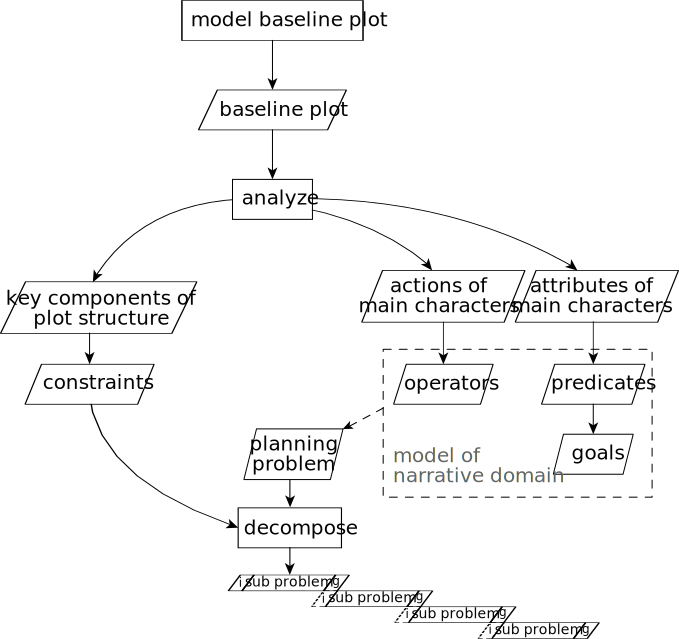
\includegraphics[scale=0.6]{discourse_model}
 \caption{Visualization of the modeling process.}
 \label{fig:modproc}
\end{figure}

Similar to the story world modeling in section \ref{fabula} attributes and actions of characters are translated into predicates and operators. Together with the goal built upon predicates this forms the model of narrative domain which leads to the initial planning problem. The chosen subset of constraints is then used to decompose the planning problem into several sub problems where the goal of a problem $n$ is the initial state of the problem $n+1$. This practice of decomposition accomplishes two things. First, since the constraints used are always different it leads to variation in the output; second, it allows for quick replanning which is necessary in the event of intervention --- i.e. when the system is used for interactive story planning.

The remaining key aspect, that is not visible in figure \ref{fig:modproc}, is PoV. It is another device for introducing variation to the story and works as follows. As one would excpect from the name, a character's \emph{point of view} renders the story from their perspective. In addition to that PoV is used to define a character's standpoint or disposition with regard to certain story events. To illustrate both aspects consider the following example: the sealing of the bond over the loan in the \emph{pound of flesh} sub-plot can be presented from the perspective of either of the involved characters, Shylock or Antonio. Furthermore let each character have two possible dispositions concerning the event. In \cite{Porteous10} the four resulting PoVs are described as follows:\\
\\
\begin{tabular}{|p{4.5cm}|p{8.5cm}|}
\hline
PoV & Action \\
\hline\hline
$(pov\ antonio\h risk\h taker)$ & Antonio, carfree risk taker, borrows money with no heed to the consequences.\\
\hline
$(pov\ antonio\h victim)$ & Antonio, a loyal friend, borrows money from Shylock, fully aware of the risks.\\
\hline
$(pov\ shylock\h victim)$ & Shylock, a patient victim, extends a favour to Antonio by lending him money.\\
\hline
$(pov\ shylock\h ruthless)$ & Shylock, intent on revenge, lends money to Antonio anticipating the forfeit.\\
\hline
\end{tabular}\\
\\
With these the sealing of the bond can be shown in 4 different ways. As a consequence the action of sealing the bond (i.e. the operation which will be part of the resulting ''story plan'') has to be defined in 4 different ways. In PDDL3.0 these are (shortened):
\begin{lstlisting}[frame=single,basicstyle=\scriptsize]
(:action borrow-money-confident-repay antonio shylock venice-rialto) ...
    :precondition   (and (pov antonio-risk-taker) ...)
    :effect         (and (sealed-bond-over-loan shylock antonio)
                    (unconcerned-over-forfeit antonio) ... ))
(:action borrow-money-wary-of-risk antonio shylock venice-rialto) ...
    :precondition   (and (pov antonio-victim) ...)
    :effect         (and (sealed-bond-over-loan shylock antonio)
                    (concerned-over-forfeit antonio) ...))
(:action lend-money-as-favour shylock antonio venice-rialto) ...
    :precondition   (and (pov shylock-victim) ... )
    :effect         (and (sealed-bond-over-loan shylock antonio) ...))
(:action (lend-money-intent-on-revenge shylock antonio venice-rialto) ...
    :precondition   (and (pov shylock-ruthless) ...)
    :effect         (and (sealed-bond-over-loan shylock antonio) ...))
\end{lstlisting}
It can be seen that $(sealed\h bond\h hover\h loan\ shylock\ antonio)$ is always an effect while other, varying effects may also be present. Furthermore PoVs are used as preconditions, ensuring that each represenation of the action is only used in plans where the corresponding PoV has been chosen.% constraints have PoV information
% PoV does two things:
%   1. show story from perspective of respective character
%   2. define character's standpoint with regard to certain events
% "different representations for the same narrative action depeding on PoV"

% - narrative control knowlege
%     -> state trajectory constraints (mention Landmarks here)
% (- interactivity) really part of approach?
% - sequence of sub problems etc. (see figure)
% - non-linear plot by identifying different possible standpoints and ranges of actions
%     -> PoV for proper variations of story
% - necessary enabling conditions (?)
% - constraints used for decomposition (figure)
%     -> selection of constraints -> variation (dynamically handeled)
\subsubsection{Result}
Clearly evident due to the inclusion of PoV this approach to narrative generation produces a discourse as a result --- that is, a solution to a planning problem representing what a viewer of the play that seved as an example might see. (TODO: Fig. 7 from Porteous paper in appendix or just mention? Mention run-time performance results?)
% - variation
% - response time
